\chapter{Crash course in Sobolev Spaces}

\label{chap-sobolev}
\section{Introduction}

Sobolev spaces are fundamental in the analysis of partial differential equations and also for 
finite element methods. Many books provide a detailed and comprehensive analysis of these spaces
that in themselves deserve significant attention if one wishes to understand the foundation that
the analysis of partial differential equations relies on. In this chapter we will however not
provide a comprehensive mathematical description of these spaces, but rather try to provide 
insight into their use. 

We will here provide the definition of these spaces. Further we will show typical functions, useful
for finite element methods,  that are in some but not all spaces. We also show how different norms
capture different characteristics.   

\section{Norms, inner products and Sobolev spaces}

Sobolev spaces are generalizations of $L^p$ spaces. $L^p$ spaces are function spaces defined as follows.  
Let $u$ be a scalar valued function on the domain $\Omega$, which for 
the moment will be assumed to be the unit interval $(0,1)$. Then the $L^p$ norm on $\Omega$ is:    
\[
\|u\|_p = (\int_0^1 |u|^p \, dx)^{1/p} .    
\]
$L^p(\Omega)$ consists of all functions for which $\|u\|_p < \infty$. 
Sobolev spaces generalize $L^p$ spaces by also including the derivatives.  
On the unit interval, the $W^{k,p}$ norm is defined as  
\begin{equation}
\label{Wpk}
\|u\|_{p,k} = (\int_\Omega \sum_{i \le k} |(\frac{\partial u}{\partial x})^i |^p \, dx)^{1/p} .    
\end{equation}
Then the Sobolev space $W^p_k(\Omega)$ consists of 
all functions with $\|u\|_{p,k} < \infty$. $W^p_k$ is a so-called Banach space - that is 
a complete\footnote{We will not go into the details of complete spaces in this book, but remark that
the space of real numbers is complete, while the space of rational numbers is not. } normed vector space. 
The corresponding semi-norm, that only include the highest order derivative is 
\begin{equation}
\label{semiWpk}
|u|_{p,k} = (\int_\Omega \sum_{i = k} |(\frac{\partial}{\partial x})^i   u|^p \, dx)^{1/p} .    
\end{equation}
The case $p=2$ is special in the sense that not only a norm is defined but also an inner product.    
The Banach space then forms a Hilbert space and these named with $H$ in Hilbert's honor. 
That is $H^k(\Omega) = W^{2,k}(\Omega)$. The inner product between the functions $u$ and $v$ is:  
\[
	(u, v)_{k} = \sum_{i \le k} \int_\Omega (\frac{\partial u}{\partial x})^i (\frac{\partial v}{\partial x})^i \,  dx.    
\]

For the most part, we will employ the two spaces $L^2(\Omega)$ and $H^1(\Omega)$, but also $H^2$ and $H^{-1}$ 
will be used. The difference between the norm in $L^2(\Omega)$ and $H^1(\Omega)$ is illustrated in the following example.   

\begin{example}{Norms of $sin(k \pi x)$} \label{sc:ex1} 
Consider the functions $u_k = \sin(k \pi x)$ on the unit interval. Figure \ref{fig:sin} shows the function for $k=1$ and $k=10$. Clearly, the $L^2$ and $L^7$ behave similarly in the sense
that they remain the same as $k$ increases. On the other hand, the $H^1$ norm of $u_k$
increases dramatically as $k$ increases. The following code shows how the 
norms are computed using FEniCS.         

\begin{python}
from dolfin import *

N = 10000 
mesh = UnitInterval(N)
V = FunctionSpace(mesh, "Lagrange", 1)

for k in [1, 100]: 
  u_ex = Expression("sin(k*pi*x[0])", k=k)
  u = project(u_ex, V)

  L2_norm = sqrt(assemble(u**2*dx))
  print "L2 norm of sin(%d pi x) %e " % (k, L2_norm) 

  L7_norm = pow(assemble(abs(u)**7*dx), 1.0/7)
  print "L7 norm of sin(%d pi x) %e " % (k, L7_norm) 

  H1_norm = sqrt(assemble(u*u*dx+inner(grad(u), grad(u))*dx))
  print "H1 norm of sin(%d pi x) %e" % (k, H1_norm) 
\end{python}

\begin{table}[h]
\begin{center}
\begin{tabular}{|c|c|c|c|}  \hline
$k \backslash norm $ & $L^2$ &   $L^7$ &  $H^1$ \\ \hline
1 & 0.71 &    0.84   & 2.3      \\ \hline
10  & 0.71 &   0.84    & 22    \\ \hline
100  & 0.71 &   0.84  &  222   \\ \hline
\end{tabular}
\caption{ The $L^2$, $L^7$, and $H^1$ norms of $sin(k \pi x)$ for k=1, 10, and 100.   }
\label{norms}
\end{center}
\end{table}


\end{example}



\begin{figure}
\label{fig:sin}
\begin{center}
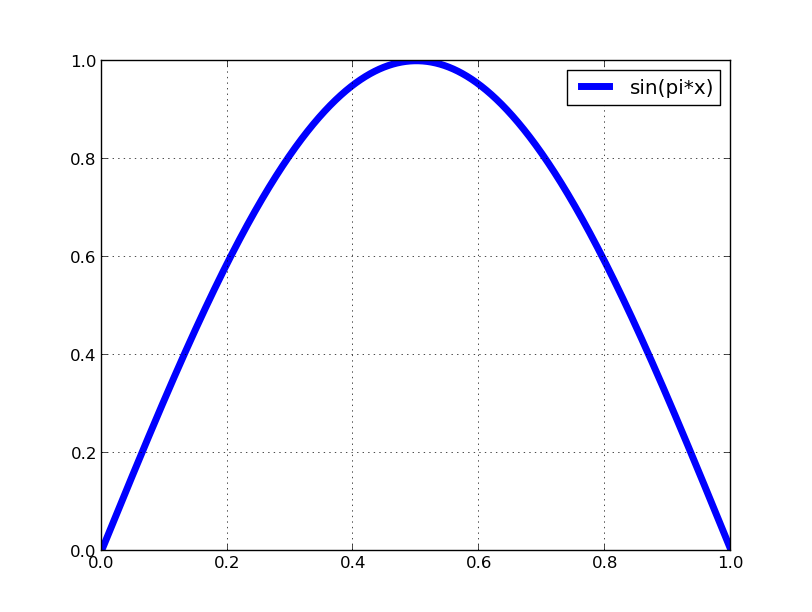
\includegraphics[width=5cm]{chapters/SobolevCrash/sin.png}
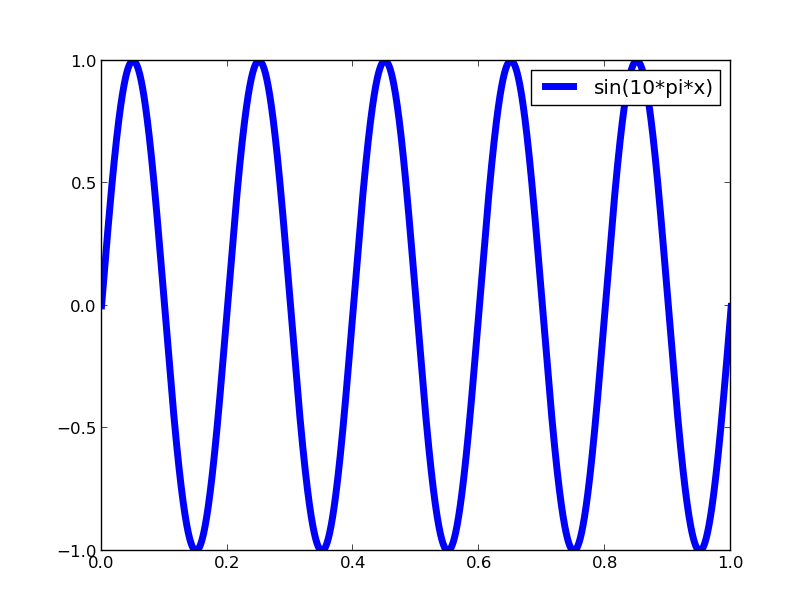
\includegraphics[width=5cm]{chapters/SobolevCrash/sin10.png}
\caption{Left picture shows $\sin(\pi x)$ on the unit interval, while 
the right picture shows $\sin(10 \pi x)$. }\label{fig:sin}
\end{center}
\end{figure}


\section{Spaces and sub-spaces, norms and semi-norms}

The Sobolev space with $k$ derivatives in $L_2(\Omega)$ was denoted by $H^k(\Omega)$. The subspace
of $H^k$ with $k-1$ derivatives equal to zero at the boundary is denoted 
$H^k_0(\Omega)$. For example, $H^1_0(\Omega)$ consists of all functions in $H^1$ that are zero 
at the boundary. Similarly, we may also defined a subspace  
$H^1_g(\Omega)$ which consists of all functions in $H^1(\Omega)$ that are equal to the function $g$ 
on the boundary. 

The norm $\|\cdot\|_{p,k}$ defined in \eqref{Wpk} is a norm
which means that $\|u\|_{p,k} > 0$ for all $u\not=0$.    
On the other hand  $|\cdot|_{p,k}$ is a semi-norm, meaning 
that $|u|_{p,k} \ge  0$ for all $u$.   
The space $H^1(\Omega)$ is defined by the norm 
\[
\|u\|_1 = (\int_\Omega u^2 + (\nabla u)^2 \, dx)^{1/2}  
\]
and contains all functions for which $\|u\|_1 \le \infty$. 
Often we consider subspaces of $H^1$ satisfying the Dirichlet boundary conditions. 
The most common space is denoted $H^1_0$. This space contains all functions 
in $H^1$ that are zero on the boundary.  
The semi-norm $|\cdot|_1$ defined as 
\[
|u|_1 = (\int_\Omega  (\nabla u)^2 \, dx)^{1/2}  
\]
is a norm on the subspace $H^1_0$. In fact, as we will see later, Poincare's lemma
ensures that $\|\cdot\|_1$ and  $|\cdot|_1$ are equivalent norms on $H^1_0$ (see Exercise \ref{ex:poincare}).  





\section{Examples of Functions in Different Spaces}

The above functions $\sin(k \pi x)$ are smooth functions
that for any $k$ are infinitely many times differentiable. 
They are therefore members of any Soblev space. 

On the other had, the step function in upper picture in Figure \ref{fig:piecewise} is 
discontinuous in $x=0.2$ and $x=0.4$. Obviously, the function is in $L^2(0,1)$, but 
the function is not in $H^1(0,1)$ since the derivative of the function  consists of Dirac's 
delta functions\footnote{The Dirac's delta function $\delta_x$ is 0 everywhere except at 
$x$ where it is  $\infty$ and $\int_\Omega \delta_x \, dx = 1$. Hence, 
Dirac's delta function is in $L^1(\Omega)$ but not in $L^2(\Omega)$.  
} 
that are $\infty$ at $x=0.2$ and 
$-\infty$ in $x=0.4$. 

The hat function in the lower picture in Figure \ref{fig:piecewise} is a typical
first order finite element function. The function is in both $L^2(0,1)$ and $H^1(0,1)$ (see
Exercise \ref{ex:piecewise}).         
In general, functions in $H^q(0,1)$ are required to be in $C^{q-1}(0,1)$, where $C^k(0,1)$ is the
class  where the $k$'th derivatives exist and
are continuous on the unit interval.   

\begin{remark}
In $C^k(\Omega)$ a function and its $k$ derivatives can be evaluated at any given point in $\Omega$ and  
the result will be a finite value. How about functions in $H^k(\Omega)$? In general only functions
in $H^k(\Omega)$ for $k\ge 2$ allow pointwise evaluation. The exact relationship between 
continous functions and Sobolev spaces are covered by the  Sobolev Embedding Theorem, which will not 
be covered in this book. 
Anyways, in $L^2(\Omega)$ or $H^1(\Omega)$ we should make note and be careful when we perform pointwise evaluations. 
\end{remark}


\begin{figure}
\begin{center}
%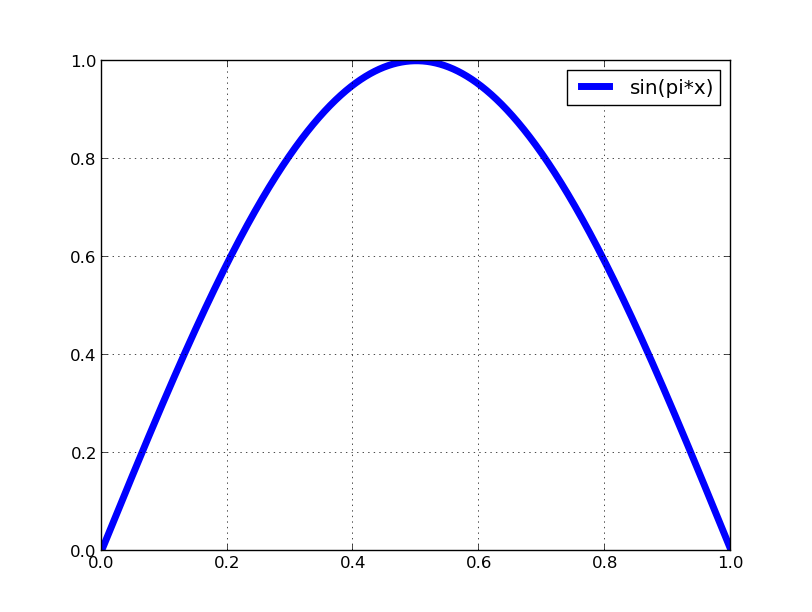
\includegraphics[width=6cm]{chapters/SobolevCrash/sin.png}
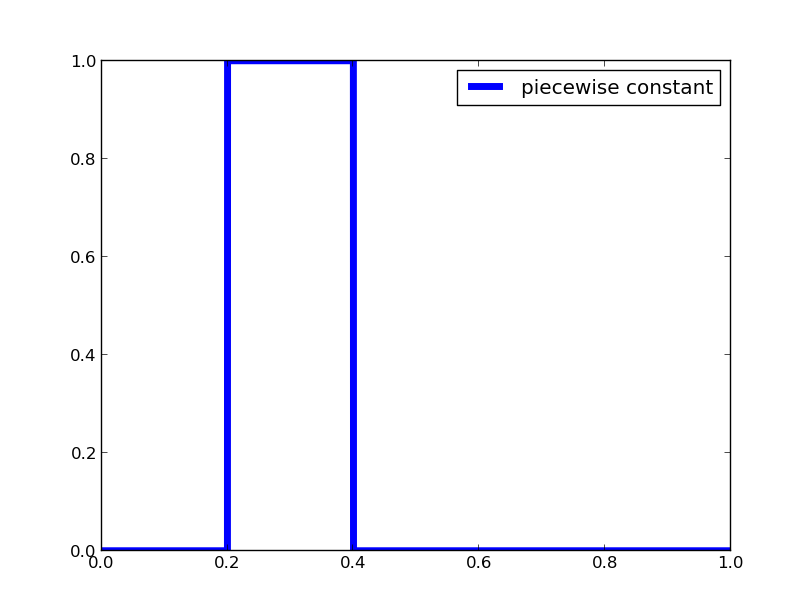
\includegraphics[width=6cm]{chapters/SobolevCrash/pc.png}
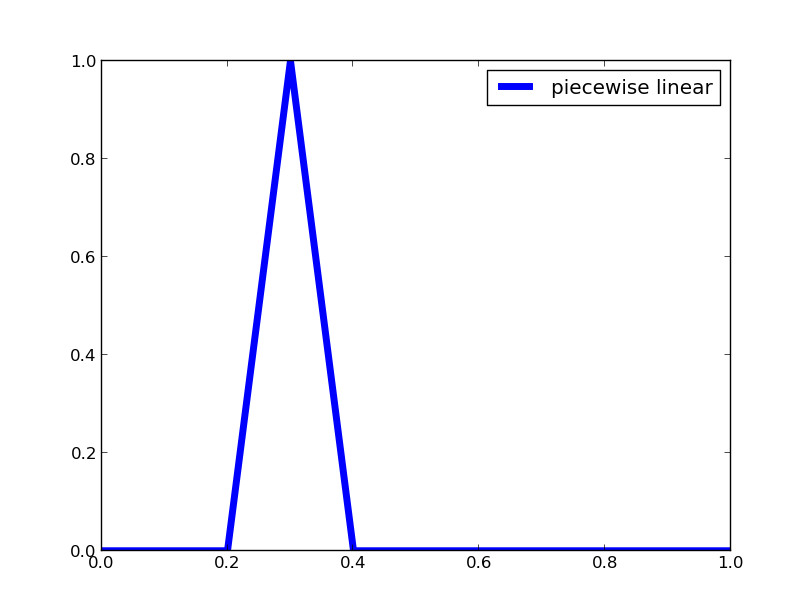
\includegraphics[width=6cm]{chapters/SobolevCrash/pl.png}
\caption{The upper picture shows a piecewise function, discontinuous at $x=0.2$ and $x=0.2$, while
the lower picture shows a linear function that is continuous. }  
\label{fig:piecewise}
\end{center}
\end{figure}

\section{Sobolev Spaces and Polynomial Approximation}
From Taylor series approximation we know that  $f(x+h)$ may be approximated
by $f(x)$ and a polynomial in $h$ that depends on the derivatives of $f$. 
To be precise, 
\[
|f(x+h) - P_{h,k} f (x) |  \le  \mathcal{O}(h^{k+1}) .    
\]
Here, $P_{h,k} f(x)$ is the following polynomial of degree $k$ in $h$, 
\[
P_{h,k} f(x) = f(x) + \sum_{n=1}^k \frac{f^{(n)}(x)}{n!} h^n . 
\]
where $f^{(n)}$ denotes the $n$'th derivative of $f$. 

In general, approximation by Taylor series bears strong requirement on the smoothness 
of the solution which needs to be differentiable in a point-wise sense.   
However, in Sobolev spaces we have the very useful approximation property  
\begin{equation}
\label{bramblehilbert}
|u - P_m u|_{k,p} \le C h^{m-k} |u|_{m,p} \quad \mbox{ for } k=0,\ldots,m \mbox{ and }  p\ge 1. 
\end{equation}
This property is used extensively in analysis of finite element methods and
is called the Bramble-Hilbert lemma for $k\ge 2$. The case $k=1$ was included by a special interpolation operator by 
Clement, the so-called Clement interpolant. 
For proof, see e.g. \cite{braess2007finite, brenner2008mathematical}.  




\section{Eigenvalues and Finite Element Methods}
\label{sec:eig and fem}

It is well known that for $-\Delta$ on the unit interval
$(0,1)$, the eigenvalues 
and eigenvectors
are $(\pi k)^2$ and $sin(\pi k x)$, $k=1, \ldots, \infty$, respectively. 
It is natural to expect that the eigenvalues in the discrete setting
approximate the continuous eigenvalues such that 
the minimal eigenvalue is $\approx \pi^2$, while the maximal eigenvalue
is $\approx \pi^2 /h^2$, where $k=1/h$ is the largest $k$ that may be represented
on a mesh with element size $h$.  
Computing the eigenvalues of the finite element stiffness matrix in FEniCS as\footnote{
We use the \emp{assemble\_system} function to enforce the Dirichlet
condition in symmetric fashion.}, 
\begin{python}
A = assemble_system(inner(grad(u), grad(v))*dx, Constant(0)*v*dx, bc)
\end{python}
reveals that the eigenvalues are differently scaled. In fact, the minimal 
eigenvalue is $\approx \pi^2 h$ and that the maximal eigenvalue is  $\approx \pi^2/h$.      
The reason is that the finite element method introduces a mesh-dependent 
scaling due to the fact that it is a variational method. 
Specifically, if we want to approximate a $f$ as $\sum_j f_j N_j$ we notice
that we may calculate $f_j$ in a variational sense as follows: 
\[
\int_\Omega \sum_j f_j N_j N_i \, dx = \int_\Omega f N_i \, dx   
\]
Hence, we notice here that, we are solving a linear system
\[
	M f = b, \mbox{ with } M_{ij} = \int_\Omega N_j N_i \, dx \mbox{ and } b_i = \int_\Omega f N_i \, dx  
\]
Both $\{f_i\}_i$ and $\{b_i\}_i$ are representations of $f$, often called the nodal and dual representations~\cite{mardal2011preconditioning}. They scale differently since
the entries of the mass matrix scale with the size of the elements in the mesh. 

To estimate the continuous eigenvalues, we  need to make sure that both the left- and right-hand sides are in the same representation, either nodal
or dual. Hence, we consider the generalized eigenvalue problem, 
\begin{equation} 
\label{geneig}
A x = \lambda M x,   
\end{equation} 
where $A$ is the above mentioned stiffness matrix and $M$ is the mass
matrix (or the finite element identity matrix) 
\begin{python}
M = assemble_system(inner(u*v*dx, Constant(0)*v*dx, bc)
\end{python}

Figure \ref{geneig} shows the eigenvalues of $-\Delta$, $A$, and  
\eqref{geneig} based on the following code: 
\begin{python}
from dolfin import *
import numpy
from scipy import linalg, matrix

def boundary(x, on_boundary): return on_boundary

for N in [100, 1000]: 
  mesh = UnitIntervalMesh(N)
  V = FunctionSpace(mesh, "Lagrange", 1)
  u = TrialFunction(V)
  v = TestFunction(V)

  bc = DirichletBC(V, Constant(0), boundary)
  A, _ = assemble_system(inner(grad(u), grad(v))*dx, Constant(0)*v*dx, bc)
  M, _ = assemble_system(u*v*dx, Constant(0)*v*dx, bc)

  AA = matrix(A.array())
  MM = matrix(M.array())

  k = numpy.arange(1, N, 1)
  eig = pi**2*k**2 

  l1, v  = linalg.eigh(AA)
  l2, v  = linalg.eigh(AA, MM)

  print "l1 min, max ", min(l1), max(l1) 
  print "l2 min, max ", min(l2), max(l2) 
  print "eig min, max ", min(eig), max(eig) 

  import pylab 
  pylab.loglog(l1[2:], linewidth=5) # exclude Dirichlet values 
  pylab.loglog(l2[2:], linewidth=5) # exclude again 
  pylab.loglog(eig, linewidth=5)
  pylab.legend(["eig(A)", "eig(A,M)", "cont. eig"], loc="upper left")
  pylab.show()
\end{python}

\begin{figure}
\begin{center}
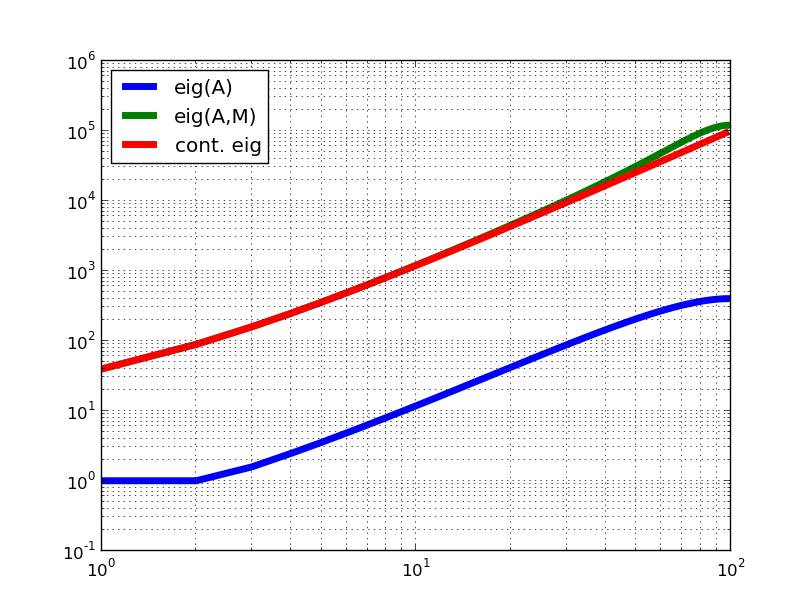
\includegraphics[width=6cm]{chapters/SobolevCrash/eig.png}
\caption{A log-log plot of the eigenvalues of $A$, $M^{-1} A$, and $-\Delta$. }  
\label{fig:geneig}
\end{center}
\end{figure}
From Figure \ref{fig:geneig} we see that that the eigenvalues
of \eqref{geneig} and $-\Delta$ are close, while the eigenvalues
of $A$ is differently scaled.  
We remark that we excluded the two smallest eigenvalues in the discretized problems 
as they correspond to the Dirichlet conditions. 
%We remark 
%that we use \emp{pytave}, the Python interface of Octave because
%\emp{numpy} is not trustworthy for eigenvalue computations on 
%"large" linear systems. A description of \emp{pytave} is found in~\cite{mardal2013combining}.  


\section{Boundary conditions, Traces and Fractional Sobolev Spaces }

In order to make sense of for instance boundary conditions we need to 
restrict from a domain $\Omega$ to $\partial \Omega$. Hence, for instance
if $\Omega$ is the unit square in 2D then $\partial \Omega$ consists of the 1D lines that 
connect the vertices at the boundary of the unit square. However, a 
1D line is inifinitely thin and has no measure in 2D. In Sobolev spaces, which
have extra smoothness in terms of the extra derivatives, the   
values at lower dimentional manifolds may be used. In fact, their use is required 
in terms of boundary conditions. In order to make sense of values at lower 
dimensional manifolds we need the mathematical constructs of traces and fractional 
Sobolev spaces. Specifically, let $T:\Omega \rightarrow \partial \Omega$ be the 
the so-called trace operator and $u \in H^k(\Omega)$ then 
$Tu \in H^{k-1/2} (\partial \Omega)$. Typically, when finite element methods
are used for single-physics problems then there is no need to pay attention to 
the fractional norms when implementing the boundary conditions. Boundary conditions
are assigned at the boundary in a straightforward way as will be discussed in the next
chapter. However, for multi-physics problems, care may be required for efficient and
accurate simulation.   

\section{Negative and Fractional Norms}

As will be discussed more thoroughly later, 
$-\Delta$ is a symmetric positive operator and can be thought of 
as an infinite dimensional matrix that is symmetric and positive.  
It is also know from Riesz representation theorem that if
$u$ solves the problem
\begin{eqnarray*}
-\Delta u &=& f, \quad \mbox{ in } \Omega, \\   
        u &=& 0, \quad \mbox{ on } \partial \Omega  
\end{eqnarray*}
then 
\begin{equation}
\label{riesz}
|u|_1 = \|f\|_{-1} . 
\end{equation}
This implicitly define the $H^{-1}$ norm, although
the definition then requires the solution of a Poisson problem.   
For example, in the previous example where
$u_k = sin(k\pi x)$, we  have already estimated  
that $|u_k|_1 = \frac{\pi k}{\sqrt{2}}$ and therefore 
$\|u_k\|_{-1} = |(-\Delta)^{-1} u_k|_1 = \frac{1}{\sqrt{2} k \pi }$.  
We notice that the $\|\cdot\|_1$ norm weights high frequency oscillations heavily (linear in $k$), whereas
the $\|\cdot\|_{-1}$ does not (it scales as $1/k$). On the other hand $L^2$ weights oscillations at all frequencies
equally.   \label{sinkpnorms} 

Let us now generalize these considerations and  consider a matrix 
(or differential operator) $A$ which is
symmetric and positive. $A$ has positive and real
eigenvalues and defines an inner product which may
be represented in terms of eigenvalues and eigenfunctions. Let     
$\lambda_i$ and $u_i$ be the eigenvalues and eigenfunctions
such that 
\[
A u_i = \lambda_i u_i  
\]
Then, $x$ may be expanded in terms of the eigenfunctions $u_i$ as
$x=\sum_i c_i u_i$, where $c_i = (x, u_i)$,  and we obtain 
\[
(x,x)_A = (A x, x) = (A \sum_i c_i u_i  , \sum_j c_j u_j)     
= (\sum_i \lambda_i  c_i u_i  , \sum_j c_j u_j)  
\]
Because $A$ is symmetric, the egenfunctions $u_i$  are orthogonal to each other
and we may choose a normalized basis such that $(u_i, u_j) =  \delta_{ij}$.
With this normalization, we simply obtain
\[
\|x\|_A^2 = (x,x)_A = (A x, x) = (A \sum_i c_i u_i  , \sum_j c_j u_j)     
= \sum_i \lambda_i  c_i^2    
\]


A generalization of the $A-$inner product (with corresponding norm) to 
a $A^q-$inner product that allow for both negative and franctional $q$  
is then as follows
\begin{equation}
\label{qnorm}
\|x\|_{A,q}^2 =  (x,x)_{A,q} =  \sum_i \lambda^q_i c_i^2.     
\end{equation}
Clearly, this definition yields 
that $|u_k|_1 = \frac{\pi k}{\sqrt{2}}$ and 
$\|u_k\|_{-1} = \frac{1}{\sqrt{2} k \pi }$, as above.  

As mentioned in Section \ref{sec:eig and fem}, 
care has to be taken in finite element methods if the discrete eigenvalues
are to correspond with the continuous eigenvalues. We will therefore detail
the computation of negative and fractional norms in the following.   
Let $\lambda_i$ and $u_i$ be the eigenvalues and eigenvectors of the following
generalized eigenvalue problem  
\begin{equation}
\label{gen_eig}
A u_i = \lambda_i M u_i 
\end{equation}
and let $U$ be the matrix with the eigenvectors as columns. 
The eigenvalues are normalized in the sense 
that 
\[
U^T M U = I 
\]
where $I$ is the identity matrix. 
We obtain 
\[
U^T A U = \Lambda \quad \mbox{ or } \quad A = M U \Lambda (M U)^T  ,  
\]
where $\Lambda$ is a matrix with the eigenvalues $\lambda_i$ on the diagonal.  
Hence also in terms of the generalized eigenvalue problem \eqref{gen_eig}
we obtain the $A-$norm as  
\[
\|x\|^2_A = x^T MU \Lambda (MU)^T x   
\]
and  
we may define fractional and negative norms in the same manner
as \eqref{qnorm}, namely that 
\[
\|x\|^2_{A,M,q} = x^T M U \Lambda^q (MU)^T x .     
\]

Defining negative and fractional norms in terms of eigenvalues and eigenvectors 
is convenient for small scale problems, but eigenvalue problems are computationally
demanding. It may, however, be tractable on subdomains, such as surfaces or interfaces 
of larger problems. There are however more    
efficient was of computing such norms and operators, but those are beyond the scope of this
book. 


\begin{example}{Computing the $H^1$, $L^2$, and $H^{-1}$ norms} \label{sc:ex2} 

Let us consider $\Omega = (0,1)$ and $u_k = sin(\pi k x)$.  
Table \ref{norms} shows the $H^1$, $L^2$, and $H^{-1}$ norms as computed
with \eqref{qnorm} with $q=1, 0$, and $-1$, respectively.  Comparing 
the computed norms with the norms $L^2$ and $H^1$ norms  computed
in Example \ref{sc:ex1}, or analytically on page \pageref{sinkpnorms}  we see that the above definition \eqref{qnorm}
reproduces the $H^1$ and $L^2$ norms with $q=1$ and $q=0$, respectively.     
We also remark that while the $H^1$ norm increases as
$k$ increases, the  $H^{-1}$ norm demonstrates a corresponding decrease.  
Below we show the code for computing these norms. 


\begin{table}[h]
\begin{center}
\begin{tabular}{|c|c|c|c|}  \hline
$k \backslash norm $ & $H^1, \ q=1  $ &   $L^2, \ q=0$ &  $H^{-1}, \ q=-1$ \\ \hline
1 &  2.2 &    0.71  &  0.22      \\ \hline
10  & 22 &    0.71   & 0.022   \\ \hline
100  & 222 &   0.71  & 0.0022   \\ \hline
\end{tabular}
\caption{ The $L^2$, $L^7$, and $H^1$ norms of $sin(k \pi x)$ for k=1, 10, and 100.   }
\label{table:norms}
\end{center}
\end{table}


\begin{python}
from dolfin import *
from numpy import matrix, diagflat, sqrt
from scipy import linalg, random 

def boundary(x, on_boundary): return on_boundary

mesh = UnitIntervalMesh(200)
V = FunctionSpace(mesh, "Lagrange", 1)
u = TrialFunction(V)
v = TestFunction(V)
bc = DirichletBC(V, Constant(0), boundary)

A, _ = assemble_system(inner(grad(u), grad(v))*dx, Constant(0)*v*dx, bc)
M, _ = assemble_system(u*v*dx, Constant(0)*v*dx, bc)
AA = matrix(A.array())
MM = matrix(M.array())

l, v = linalg.eigh(AA, MM)
v = matrix(v)
l = matrix(diagflat(l))

for k in [1, 10, 100]: 
  u_ex = Expression("sin(k*pi*x[0])", k=k)
  u = interpolate(u_ex, V)
  x = matrix(u.vector().array())

  H1_norm = pi*k*sqrt(2)/2  
  print "H1 norm of sin(%d pi x) %e (exact)          " % (k, H1_norm) 
  H1_norm = sqrt(assemble(inner(grad(u), grad(u))*dx)) 
  print "H1 norm of sin(%d pi x) %e (|grad(u)|^2)    " % (k, H1_norm) 
  H1_norm = sqrt(x*AA*x.T)    
  print "H1 norm of sin(%d pi x) %e (x A x' )        " % (k, H1_norm) 
  W = MM.dot(v)
  H1_norm = sqrt(x*W*l*W.T*x.T)   
  print "H1 norm of sin(%d pi x) %e (eig)            " % (k, H1_norm) 

  print "" 

  L2_norm = sqrt(2)/2 
  print "L2 norm of sin(%d pi x) %e (exact)          " % (k, L2_norm) 
  L2_norm = sqrt(assemble(u**2*dx)) 
  print "L2 norm of sin(%d pi x) %e   |u|^2          " % (k, L2_norm) 
  L2_norm = sqrt(x*MM*x.T) 
  print "L1 norm of sin(%d pi x) %e (x M x' )        " % (k, L2_norm) 
  W = MM.dot(v)
  L2_norm = sqrt(x*W*l**0*W.T*x.T)   
  print "L2 norm of sin(%d pi x) %e (eig)            " % (k, L2_norm) 

  print "" 

  Hm1_norm = sqrt(2)/2/k/pi  
  print "H^-1 norm of sin(%d pi x) %e (exact)        " % (k, Hm1_norm) 
  Hm1_norm = sqrt(x*W*l**-1*W.T*x.T)  
  print "H^-1 norm of sin(%d pi x) %e (eig)          " % (k, Hm1_norm) 
  Hm1_norm = sqrt(x*MM*linalg.inv(AA)*MM*x.T)    
  print "H^-1 norm of sin(%d pi x) %e (x inv(A) x') " % (k, Hm1_norm) 
\end{python}

\end{example}


\begin{remark}{\textbf{Norms for $|q| > 1$.} } \\
The norm \eqref{qnorm} is well defined for any $|q|$ > 1, but will not 
correspond to the corresponding Sobolev spaces.    
\end{remark}

\begin{remark}{\textbf{The standard definition of a dual norm}} \\
\label{dualnorm}
Let $(\cdot, \cdot)_A$ be an inner product over the Hilbert
space $V$.  The norm of the dual space is then defined by 
\[
\|f\|_{A^*} = \sup_{v\in V} \frac{(f,v)}{(v,v)_A} .    
\]
For example, the $H^{-1}$ norm is defined as 
\[
\|f\|_{-1} = \sup_{v\in H^1} \frac{(f,v)}{(v,v)_1} .    
\]


\end{remark}

\section{Exercises}

\begin{exercise}
Compute the $H^1$ and $L^2$ norms of a random function with values
in $(0,1)$ on meshes representing the unit interval of with $10$, $100$, and $1000$ cells.   
\end{exercise}

\begin{exercise}
Compute the $H^1$ and $L^2$ norms of  $\sin( k \pi x)$ on the unit interval analytically 
and compare with the values presented in Table \ref{table:norms}.   
\end{exercise}

\begin{exercise}
\label{ex:piecewise}
Compute the $H^1$ and $L^2$ norms of  the hat function in Picture \ref{fig:piecewise}.   
\end{exercise}



\begin{exercise}
\label{ex:hat2}
Consider the following finite element function $u$ defined
as  
\[
u = \Bigg\{ 
\begin{array}{ll} \frac{1}{h} x - \frac{1}{h} (0.5 - h), & x=(0.5-h,0.5) \\  
              -\frac{1}{h} x + \frac{1}{h} (0.5 - h),  & x=(0.5,0.5 + h) \\  
                0, & \mbox{elsewhere}  
\end{array}
\]
That is, it corresponds to the hat function in Figure \ref{fig:piecewise}, where
$u(0.5)=1$ and the hat function is zero every where in $(0,0.5-h)$ and  $(0.5+h, 1)$.  
Compute the $H^1$ and $L^2$ norms of this function analytically, and the 
$L^2$, $H^1$ and $H^{-1}$ norms numerically for $h=10$, $100$ and $1000$.    
\end{exercise}






